\subsubsection{Storage in OpenScienceLab}

\newline
In OpenScienceLab, users have access to both ephemeral and persistent storage.

\paragraph{Ephemeral Storage}

OpenScienceLab servers run in a \href{https://www.docker.com/resources/what-container/}{Docker container} that uses a pre-built \href{https://docs.docker.com/get-started/docker-concepts/the-basics/what-is-an-image/}{Docker image}. Each user container comes with ephemeral storage containing the user's root directory.

Much of this ephemeral storage is locked down, and users cannot write to it.

\begin{framed}
\textbf{Warning}\\
Nothing written to directories above the user \texttt{home} directory (\texttt{/home/jovyan}) will persist across server restarts.
\end{framed}


\bigskip
\centerline{\rule{13cm}{0.4pt}}
\bigskip

\paragraph{Persistent Storage}

OpenScienceLab users typically have access to persistent storage in all their labs, but individual lab owners determine this.

Assuming a lab has persistent storage, it occupies the user's \texttt{home} directory (\texttt{/home/jovyan}).

\begin{framed}
\textbf{Storage in OpenSARLab}\\
\begin{itemize}
\item OpenSARLab users have access to 500GB of persistent storage
\item Persistent storage is permanently deleted after 30 days of inactivity. Warning emails are sent to inactive users after 29, 27, and 24 days.
\end{itemize}
\end{framed}

\begin{framed}
\textbf{Keep track of available persistent storage space with the storage monitor}\\
\begin{figure}[!htbp]
\centering
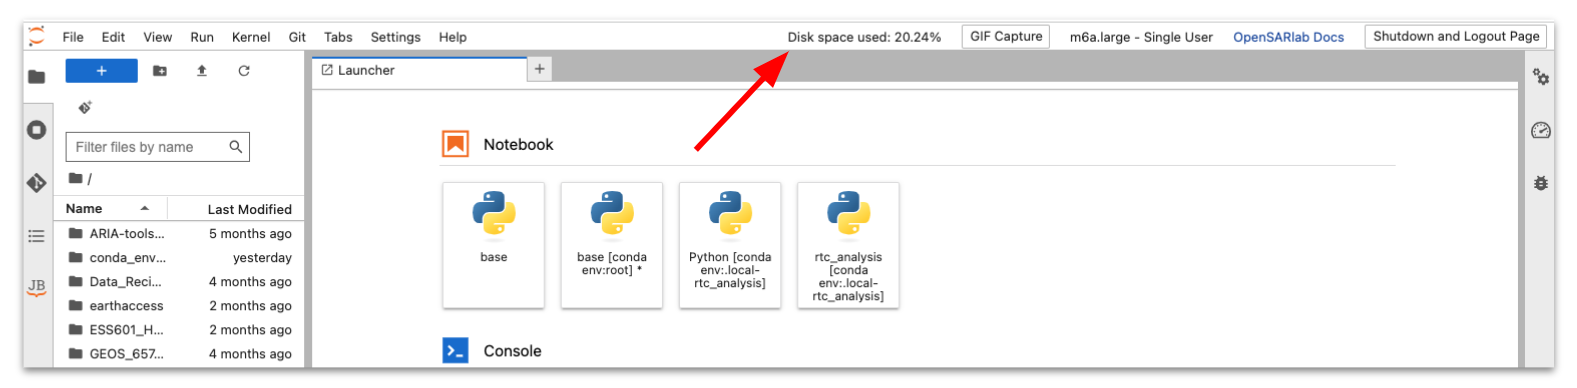
\includegraphics[width=0.7\linewidth]{files/storage_monitor-adefe078b91a683b2d14724e1b331377.png}
\end{figure}
\end{framed}